\chapter{Entwicklungs-Werkzeuge}

Für die Entwicklung und Dokumentation dieser Arbeit wurden unter anderem folgende Werkzeuge verwendet:
\begin{itemize}
	\item Das Android Software Development Kit von Google
	\item Eclipse mit der Android Development Tools Erweiterung von Google
	\item Google Code und Subversion
	\item LaTeX (MikTeX bzw. TeX Live)
	\item Google Docs \& Spreadsheets
	\item Inkscape
	\item Das GNU Image Manipulation Program (GIMP)
\end{itemize}

Zusätzlich wurden zur Erleichterung der Dokumentation ein paar eigene Werkzeuge behelfsmässig selber entwickelt.

\section{graphml2svg}

Um die Darstellung des Graphen automatisieren zu können, wurde als Erstes versucht, eine Transformation der GraphML-Datei in der dieser gespeichert wird in eine SVG-Bild vorzunehmen. Da beides XML-Formate sind sollte dazu XSLT verwendet.

Allerdings mussten wir feststellen, dass dieser auf diesem Artikel\cite{graphml_svg} basierende Ansatz nur sehr eingeschränkt funktionierte. Da mit XSLT nur über Rekursion gearbeitet werden kann wurde bei grösseren Graphen die maximal möglichen Rekursionsstufen der gängigen Werkzeuge relativ schnell erreicht und auch die Darstellung der Graphen war nicht ganz fehlerfrei.

\begin{figure}[h!]
   \centering
   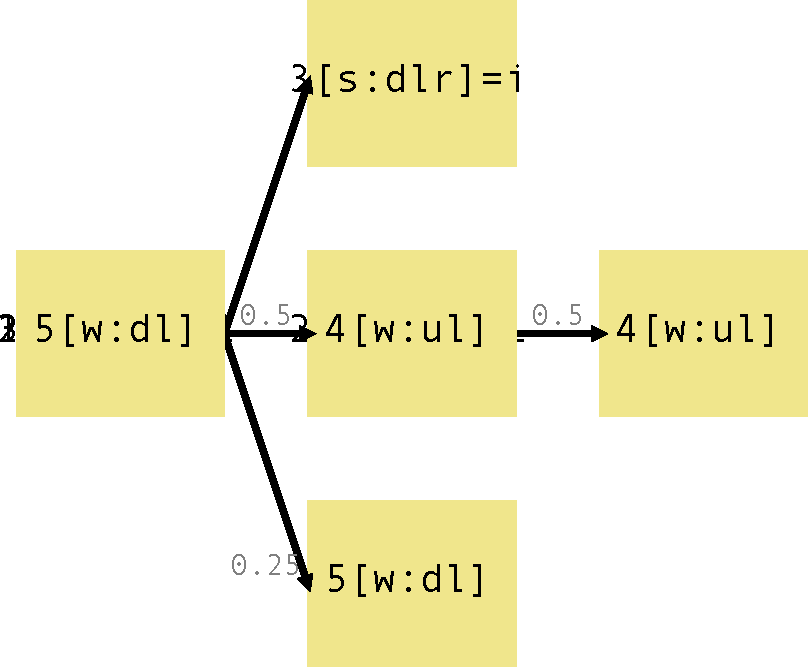
\includegraphics[scale=0.3]{img/graphml2svg} 
   \caption{Simple Beispiel-Graph konvertiert nach SVG}
   \label{fig:graphml2svg}
\end{figure}

Der Quelltext des Werkzeugs ist im Quellen-Ordner unter ./playground/graphml2svg zu finden.

\section{Graph2SVG}

Da wir den Graphen sowieso schon in Java eingelesen hatte, lag es als nächste nahe, ein rudimentäres Werkzeug zur Konvertierung des Graphen nach SVG zu schreiben. Dies gelang auch recht schnell und die resultierenden SVG-Grafiken waren auch grafisch überzeugen.

Das Programm liesst zuerst die GraphML-Datei in unsere Datenstrukturen aus dem Hauptprojekt ein und berechnet dann die Positionen der Knoten und Kanten in der Grafik und erzeugt eine entsprechende SVG-Datei.

\begin{figure}[h!]
   \centering
   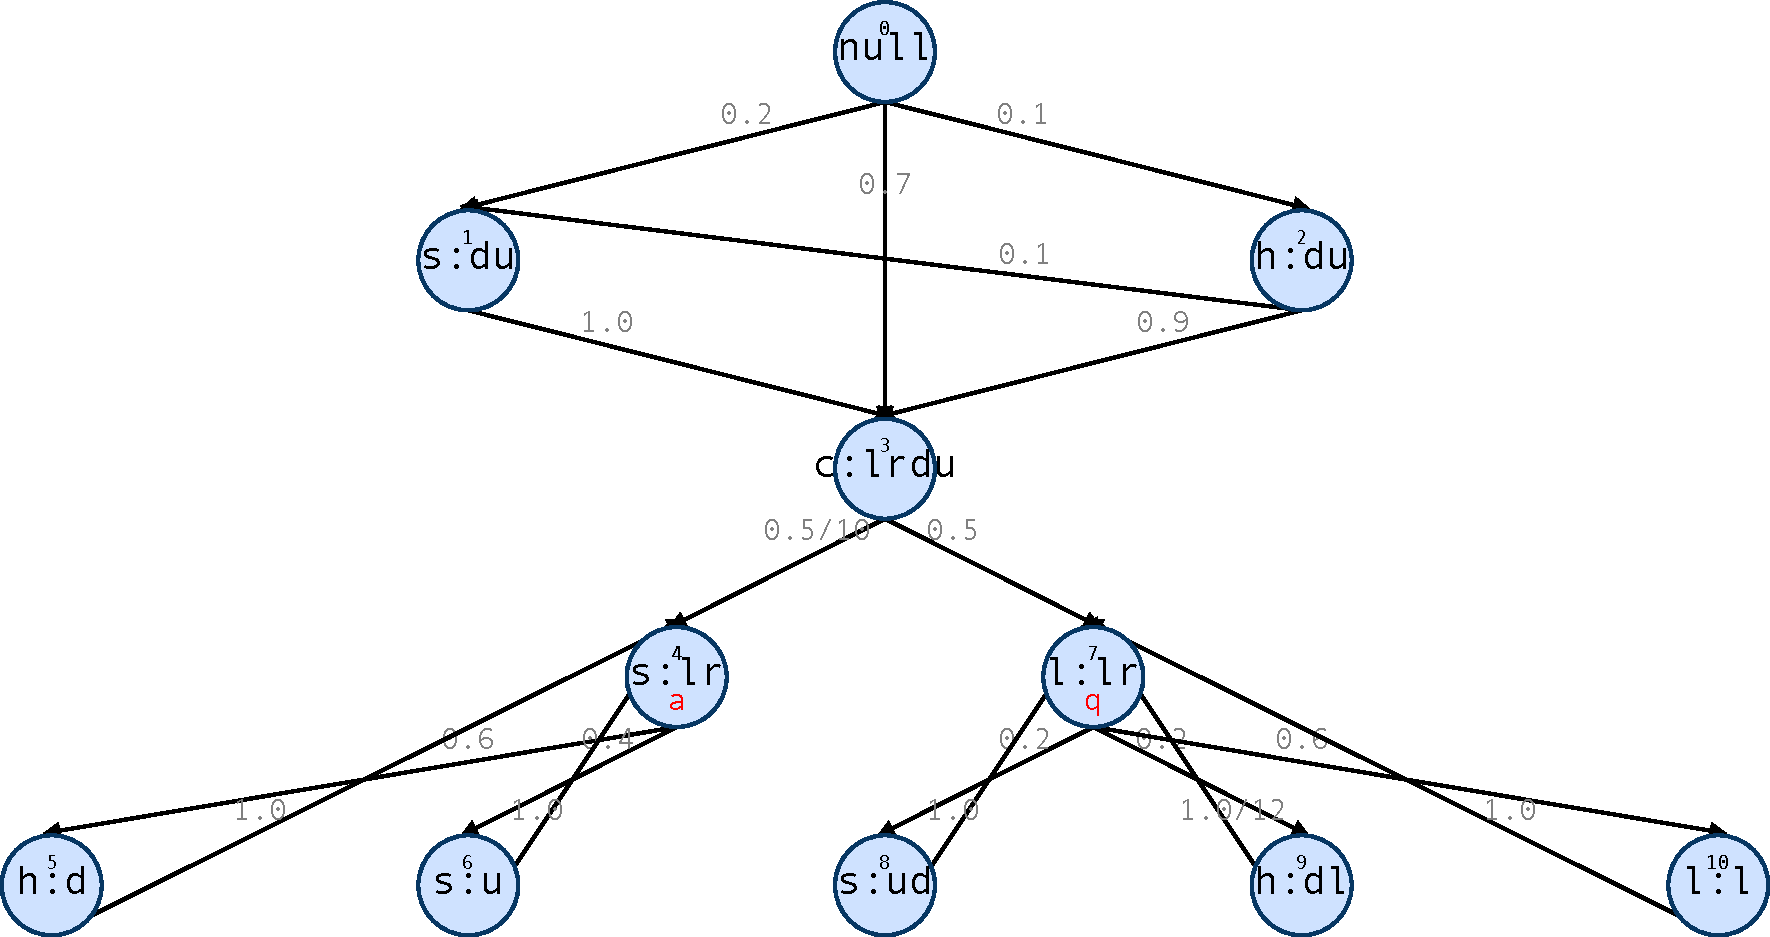
\includegraphics[width=\textwidth]{img/Graph2SVG} 
   \caption{Beispiel-Graph konvertiert nach SVG}
   \label{fig:graph2svg}
\end{figure}

Der Quelltext des Werkzeugs und eine ausführbares Jar-Archiv ist im Quellen-Ordner unter ./playground/Graph2SVG zu finden.
